\hypertarget{oppgave1}{}
\section*{Oppgave 1}
\addcontentsline{toc}{section}{Oppgave 1}

Den periodiske funksjonen er gitt som:
\[
r(t)=4\cos\left(2\pi400t+\frac{\pi}{4}\right)
+6\cos\left(2\pi800t-\frac{\pi}{2}\right).
\]

% --------------------------------------------------
\subsection*{a)}
For å skrive signalet som en sum av komplekse eksponentialledd
benyttes invers Euler-formel:
\[
\cos(\theta)=\frac{e^{j\theta}+e^{-j\theta}}{2}.
\]
Det første cosinusleddet kan dermed skrives som:
\[
    4\cos\left(2\pi400t+\frac{\pi}{4}\right)  = 4 \cdot \frac{1}{2}(e^{j(2\pi400t + \pi/4)}+e^{-j(2\pi400t + \pi/4)}).
\]
Det andre cosinusleddet blir:
\[
    6\cos\left(2\pi800t-\frac{\pi}{2}\right)
    =
    6 \cdot \frac{1}{2}(e^{j(2\pi800t-\pi/2)}+e^{-j(2\pi800t-\pi/2)}).
\]
Signalet kan derfor skrives som:
\[
\boxed{
r(t)=
2e^{j\pi/4}e^{j2\pi400t}
+
2e^{-j\pi/4}e^{-j2\pi400t}
+
3e^{-j\pi/2}e^{j2\pi800t}
+
3e^{j\pi/2}e^{-j2\pi800t}
}
\]
% --------------------------------------------------
\subsection*{b)}
Fra uttrykket i deloppgave a) ser vi at signalet har
frekvenskomponenter ved:
\[
f=\pm400\text{ Hz},\qquad f=\pm800\text{ Hz}.
\]
De komplekse koeffisientene er:
\[
\begin{array}{c|c}
f\,[\mathrm{Hz}] & C_f \\ \hline
-800 & 3e^{j\pi/2} \\
-400 & 2e^{-j\pi/4} \\
400  & 2e^{j\pi/4} \\
800  & 3e^{-j\pi/2}
\end{array}
\]
Magnitudene til frekvenskomponentene blir:
\[
    3,\qquad2,\qquad2,\qquad3.
\]
Fasene blir:
\[
\frac{\pi}{2},\qquad
-\frac{\pi}{4},\qquad
\frac{\pi}{4},\qquad
-\frac{\pi}{2}.
\]
\begin{figure}[H]
    \centering
    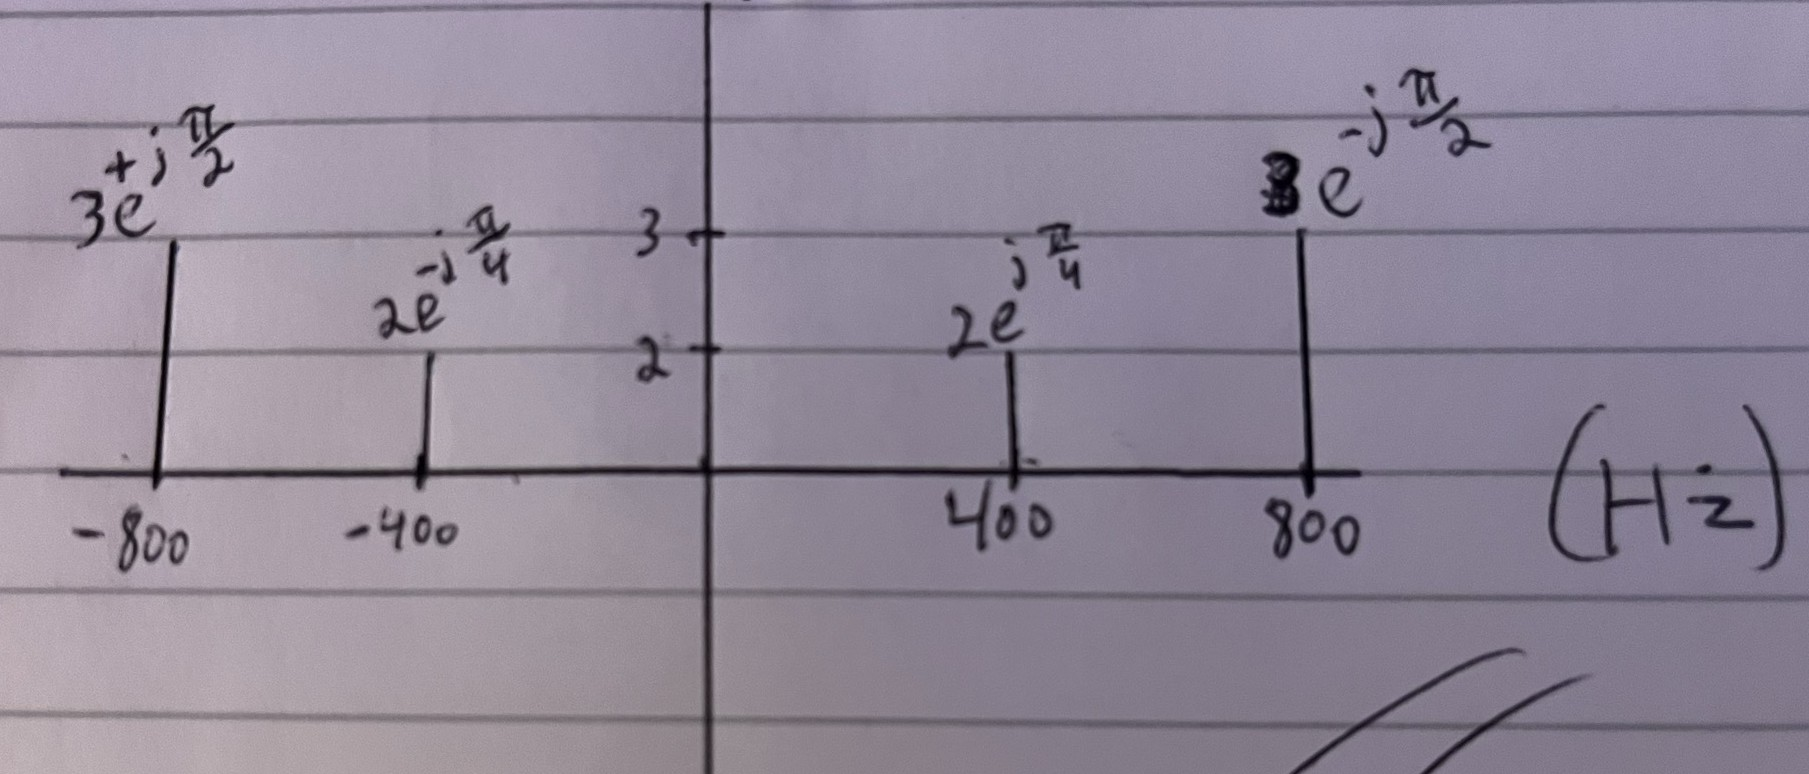
\includegraphics[width=1\textwidth]{Media/ag.jpg}
    \caption{Frekvensspekteret til signalet $r(t)$.}
    \label{fig:oppgave1b}
\end{figure}
% --------------------------------------------------
\subsection*{c)}
Signalet inneholder frekvensene 400 Hz og 800 Hz.
Begge frekvenskomponentene er heltallsmultipler av en felles grunnfrekvens:
\[
f_0= \mathrm{gcd}(400,\ 800) = 400\text{ Hz}.
\]
Dette ser vi siden:
\[
400=1\cdot400,\qquad800=2\cdot400.
\]
Signalet er derfor periodisk.
Periodetiden blir:
\[
T_0=\frac{1}{f_0}
=\frac{1}{400}
=2.5\cdot10^{-3}\text{ s}.
\]
Dermed er:
\[
\boxed{T_0=2.5\text{ ms}}.
\]